\section{Generazioni cellulari}
Nel corso degli anni, si sono susseguite diverse generazioni di tecnologie cellulari, che hanno apportato
notevoli cambiamenti alla loro architettura. Di seguito verranno presentati le principali caratteristiche
delle diverse generazioni cellulari, in modo tale da rendere di facile comprensione l'analisi dei meccanismi
di identificazione che verranno approfonditi nelle prossime sezioni.\\
Oltre ad elencare le principali caratteristiche di ogni generazione verranno analizzate nel dettaglio le specifiche  
dell'architettura di rete.
\begin{figure}[h]
    \centering
    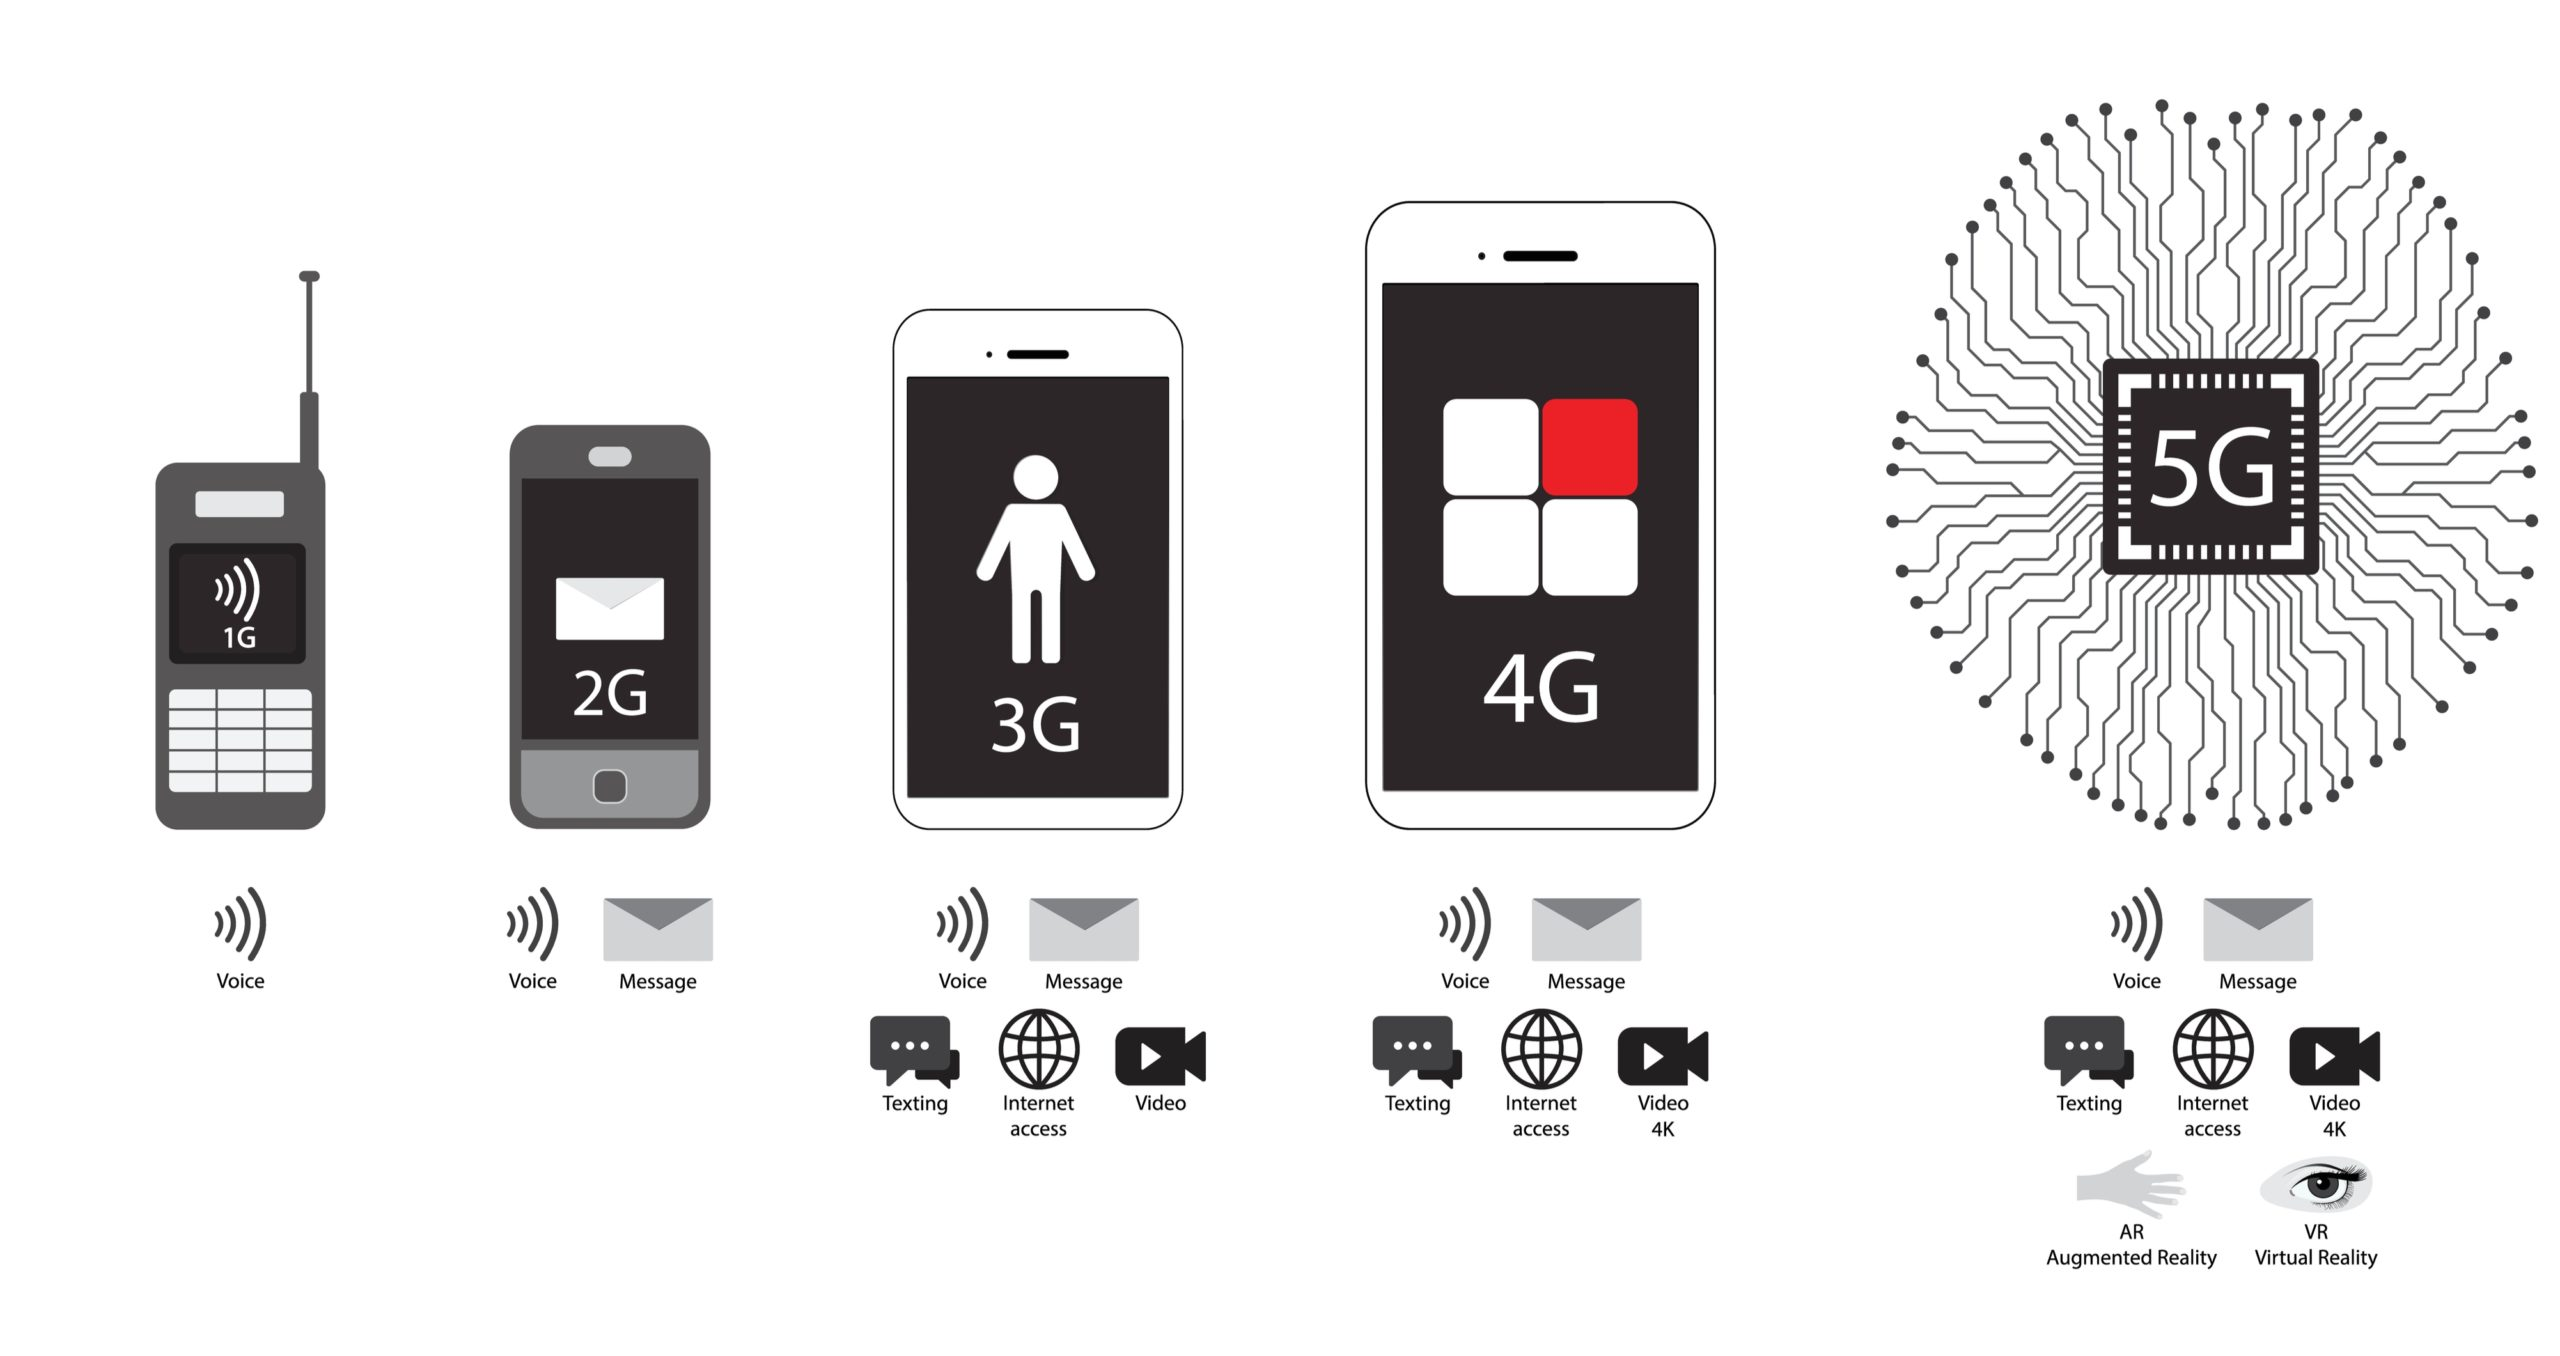
\includegraphics[width=0.7\textwidth]{images/generations-scheme.jpg}
    \caption{Schema delle generazioni cellulari}
\end{figure}

\subsection{1G}
La generazione 1G è uno dei primi standard di comunicazione cellulare. Il suo funzionamento era completamente analogico 
e ormai è stata rimpiazzata totalmente dalle generazioni successive.\\
L'architettura di questa generazione è molto semplice
\begin{figure}[h]
    \centering
    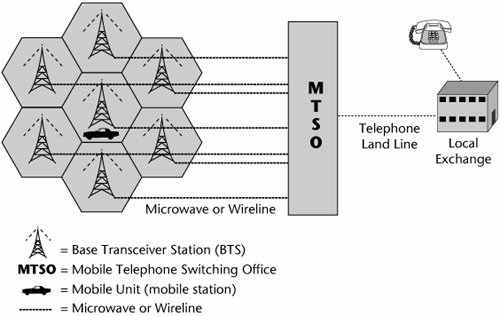
\includegraphics[width=0.7\textwidth]{images/1g.jpg}
    \caption{Architettura 1G}
\end{figure}


\subsection{2G}


\subsubsection{GSM}


\subsubsection{GPRS}


\subsubsection{EDGE}


\subsection{3G}


\subsubsection{UMTS}


\subsubsection{HSPA/HSPA+}


\subsection{4G}


\subsection{5G}